\begin{definition}[מרחק]
בהינתן גרף 
$G = (V, E)$,
נגדיר את 
\emph{המרחק}
בין שני צמתים 
$u,v \in V$,
ונסמנו 
$dist_G(u,v)$,
כמספר הקשתות המינימלי במסלול מ-$u$ ל-$v$.
\end{definition}
\noindent
\textbf{הערה:}
כאשר ברור על איזה גרף מדובר נסתפק בסימון 
$dist(u,v)$.
\vspace{5mm}
\\
\textbf{קלט:}
גרף $G$ (מכוון או לא) וצומת מקור $s$.
\\
\textbf{מטרה:}
למצוא עץ עם שורש $s$,
$T = (U, F)$, 
$U \subseteq V$, 
$F \subseteq E$
כך ש-$U$ היא קבוצת הצמתים שישיגים מ-$s$.
בנוסף, לכל צומת 
$u \in U$
מתקיים
$dist_T(s, u) = dist_G(s, u)$,
$d(u) = dist(s,u)$
ו-%
$p(u)$
יצביע לאבא של 
$u$.
\\
למשל:
\begin{center}
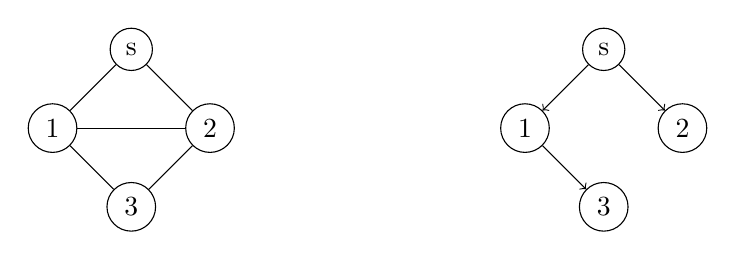
\begin{tikzpicture}[every node/.style={circle, draw, minimum width=5mm}]

\node(s) at(0,0) {s};
\foreach [count=\i] \x\y in {-1/-1,1/-1,0/-2}{
	\node(\i) at(\x,\y) {\i};
}

\foreach \u \v in {
s/1%
,s/2%
,1/2%
,1/3%
,2/3%
}{
	\draw (\u) -- (\v);
}

\begin{scope}[xshift=6cm]
\node(s) at(0,0) {s};
\foreach [count=\i] \x\y in {-1/-1,1/-1,0/-2}{
	\node(\i) at(\x,\y) {\i};
}

\foreach \u \v in {
s/1%
,s/2%
,1/3%
}{
	\draw[->] (\u) -- (\v);
}
\end{scope}

\end{tikzpicture}
\end{center}

\begin{enumerate}
\item
אתחול:
$U \leftarrow \{s\}, F \leftarrow \emptyset$, 
לכל 
$v \in V$
מציבים
$p(v) \leftarrow nil, d(v) \leftarrow \infty$,
$d(s) \leftarrow 0$
\item 
\label{item:bfs:while}
כל עוד ישנה קשת 
$uv$
שחוצה את $U$ 
($u \in U$)
בחר קשת עם 
$d(u)$
מינימלי
	\begin{enumerate}
	\item
	$U \leftarrow U \cup \{v\}, F \leftarrow F \cup \{uv\}$
	\item
	$p(v) = u$
	\item
	$d(v) = d(u) + 1$
	\end{enumerate}
\end{enumerate}
BFS
הוא מקרה פרטי של האלגוריתם הכללי.

\begin{claim}
לכל
$v \in V$
מתקיים
$d(v) \geq dist_G(s, v)$
\end{claim}
\begin{proof}
באינדוקציה על צעד האלגוריתם
\end{proof}

\begin{claim}
לכל
$v \in V$
מתקיים
$d(v) \leq dist_G(s,v)$
\end{claim}
\begin{proof}
באינדוקציה על צעד האלגוריתם
\end{proof}

\begin{claim}
לכל
$v \in V$
מתקיים
$d(v) = dist_T(s,v)$
\end{claim}
\begin{proof}
באינדוקציה על צעד האלגוריתם
\end{proof}


\begin{theorem}
לכל
$v \in V$
מתקיים
$d(v) = dist_T(s,v) = dist_G(s,v)$
\end{theorem}
\\
\noindent
מהו זמן הריצה של BFS ? קשה להגיד כי לא הגדרנו כיצד מתבצעת הבדיקה בשלב 
\ref{item:bfs:while}
של האלגוריתם. 
ניתן לממש BFS על ידי תור באופן הבא:
\begin{enumerate}
\item
אתחול:
$U \leftarrow \{s\}, F \leftarrow \emptyset$, 
לכל 
$v \in V$
מציבים
$p(v) \leftarrow nil, d(v) \leftarrow \infty$,
$d(s) \leftarrow 0, Q \leftarrow (s)$
\item 
כל עוד התור לא ריק 
\begin{enumerate}
	\item
	$u \leftarrow Q.pop()$
\item
כל עוד ישנה קשת 
$uv$
שחוצה את $U$
($u \in U$)
		\begin{enumerate}
		\item
		$U \leftarrow U \cup \{v\}, F \leftarrow F \cup \{uv\}$
		\item
		$p(v) = u$
		\item
		$d(v) \leftarrow d(u) + 1$
		\item
		$Q.push(v)$
		\end{enumerate}
	\end{enumerate}
\end{enumerate}
\\
\noindent
נשים לב שבמימוש הנ"ל כל צומת נכנסת ויוצאת מהתור לכל היותר פעם אחת 
ובנוסף כל קשת נבדקת לכל היותר פעם אחת ולכן זמן הריצה הוא 
$O(|V| + |E|)$
נשאר להוכיח שזהו אכן מימוש של BFS.
מספיק להוכיח את שתי הטענות הבאות:
\begin{claim}
כל עוד קיימת קשת שחוצה את $U$ התור לא ריק
\end{claim}
\begin{proof}
באינדוקציה על צעד האלגוריתם
\end{proof}

\begin{claim}
התור מונוטוני לא יורד בהתייחס לערכי 
$d$
\end{claim}
\begin{proof}
נוכיח טענה חזקה יותר באינדוקציה על צעד האלגוריתם: 
התור מונוטוני לא יורד וגם 
$|d(u) - d(v)| \leq 1$
לכל שני צמתים שבתור
\end{proof}
